\section{Ideal Loads Air System }\label{ideal-loads-air-system}

\subsection{Overview}\label{overview-021}

The input object ZoneHVAC:IdealLoadsAirSystem provides a model for an ideal HVAC system. It occupies a place in the program hierarchy corresponding to a zone HVAC unit. It is not connected to a central air system -- instead each ZoneHVAC:IdealLoadsAirSystem object supplies cooling or heating air to a zone in sufficient quantity to meet the zone load or up to its limits, if specified. The ideal loads air system(s) may be optionally connected to a return plenum. The supply air conditions are controlled based on specifications in the ZoneHVAC:IdealLoadsAirSystem input. The system has options for humidity control, outdoor air, economizer, demand controlled ventilation, and heat recovery.

\begin{figure}[hbtp] % fig 267
\centering
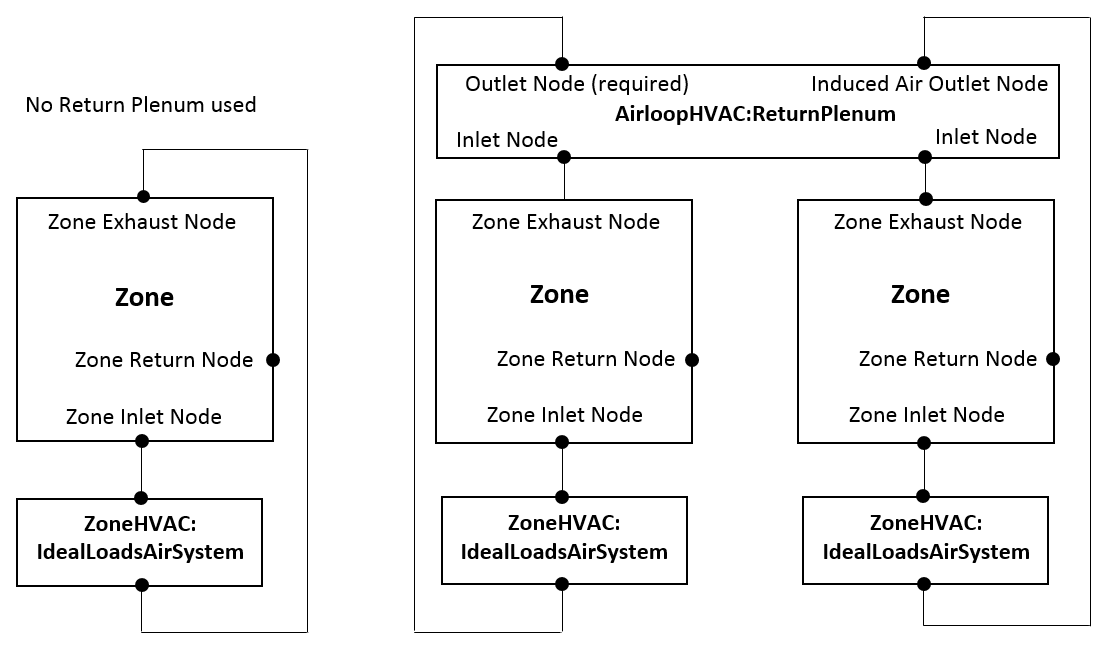
\includegraphics[width=0.9\textwidth, height=0.9\textheight, keepaspectratio=true]{media/IdealLoadsSchematic.png}
\caption{Ideal Loads Air System with and without plenum \protect \label{fig:ideal-loads-air-system-with-and-without-plenum}}
\end{figure}


\subsection{Model}\label{model-002}

The ZoneHVAC:IdealLoadsAirSystem object is modeled as an ideal VAV terminal unit with variable supply temperature and humidity. The supply air flow rate is varied between zero and the maximum in order to satisfy the zone heating or cooling load, zone humidity controls, outdoor air requirements, and other constraints, if specified.

\subsubsection{Inputs and Data}\label{inputs-and-data-002}

The user specifies some or all of the following data for each ZoneHVAC:IdealLoadsAirSystem object:

\begin{itemize}
  \item name of unit availability schedule
  \item name of the zone inlet node;
  \item name of the zone exhaust node;
  \item name of the system inlet node (if plenum is used);
  \item maximum supply air temperature when in heating mode \emph{T\(_{max,heating}\)} {[}C{]};
  \item minimum supply air temperature when in cooling mode \emph{T\(_{min,cooling}\)} {[}C{]};
  \item maximum supply air humidity ratio when in heating mode \emph{W\(_{max,humid}\)} {[}kg water/kg dry air{]};
  \item minimum supply air humidity ratio when in cooling mode \emph{W\(_{min,dehum}\)} {[}kg water/kg dry air{]};
  \item heating limit type flag (\emph{LimitFlowRate, LimitCapacity, LimitFlowRateAndCapacity} or \emph{NoLimit}) \emph{HeatingLimit};
  \item maximum heating air flow rate~ {[}m\(^{3}\)/s{]}
  \item maximum sensible heating capacity~ {[}W{]}
  \item cooling limit type flag (\emph{LimitFlowRate, LimitCapacity, LimitFlowRateAndCapacity} or \emph{NoLimit}) \emph{CoolingLimit}
  \item maximum cooling air flow rate~ {[}m\(^{3}\)/s{]}
  \item maximum total cooling capacity~ {[}W{]}
  \item name of heating availability schedule
  \item name of cooling availability schedule
  \item dehumidification control type flag (\emph{ConstantSensibleHeatRatio, Humidistat, None,} or \emph{ConstantSupplyHumidityRatio}) \emph{DehumidCtrlType}
  \item cooling sensible heat ratio
  \item humidification control type flag (\emph{Humidistat, None,} or \emph{ConstantSupplyHumidityRatio}) \emph{HumidCtrlType}
  \item name of a DesignSpecification:OutdoorAir object
  \item outdoor air inlet node name
  \item demand controlled ventilation control type flag (\emph{None, OccupancySchedule or CO2Setpoint})
  \item outdoor air economizer type flag (\emph{NoEconomizer, DifferentialDryBulb, or DifferentialEnthalpy})
  \item heat recovery type flag (\emph{None, Sensible, or Enthalpy})
  \item sensible heat recovery effectiveness
  \item latent heat recovery effectiveness
\end{itemize}

\subsubsection{All input data for the ZoneHVAC:IdealLoadsAirSystem is stored in the array PurchAir. The model and data are encapsulated in the module PurchasedAirManager.Calculation}\label{all-input-data-for-the-zonehvacidealloadsairsystem-is-stored-in-the-array-purchair.-the-model-and-data-are-encapsulated-in-the-module-purchasedairmanager.calculation}

\begin{itemize}
  \item Set the unit on/off flag \emph{UnitOn}.

    The unit is off (\emph{UnitOn} = \emph{False}) if the unit availability schedule value is \textless{} = 0; otherwise the unit is on (\emph{UnitOn} = \emph{True}). If the unit is on, the calculation proceeds through the remaining steps. If the unit is off, the zone inlet node conditions are set to the zone node condition, the inlet node mass flow rate is set to zero, and the unit outputs are set to zero.

  \item Calculate the minimum outdoor air mass flow rate based on the specifications in the DesignSpecification:OutdoorAir object, if specified.
  \item Calculate the sensible and latent impact of the outdoor air flow relative to the zone conditions
  \item Determine if the unit needs to heat or cool 
    \begin{itemize}
      \item If outdoor air sensible impact is \textgreater{} = load to zone cooling setpoint and the current thermostat type is not SingleHeatingSetPoint, then unit is in cooling mode
      \item If outdoor air sensible impact is \textless{} load to zone heating setpoint then unit is in heating mode
      \item Else if neither condition is true, then unit is in deadband mode (provides outdoor air but shuts off economizer and heat recovery and all humidity control options except \emph{Humidistat} option) 
    \end{itemize}
  \item If in cooling mode, simulate outdoor air economizer and adjust outdoor air mass flow rate
  \item Calculate supply air mass flow rate 

    \begin{itemize}
      \item If outdoor air flow rate exceeds applicable maximum flow rate (heating or cooling) then reduce outdoor air mass flow rate, issue warning, and set supply air mass flow rate equal to outdoor air mass flow rate
    \end{itemize}

    Else

    \begin{itemize}
      \item Calculate supply air mass flow rate required to meet zone sensible load at the applicable (heating or cooling) supply temperature limit (\emph{T\(_{max,heating}\)} or \emph{T\(_{min,cooling}\)})

        \begin{equation}
          {\dot m_s} = {\dot Q_z}/({c_{p,air}}\cdot ({T_s} - {T_z}))
        \end{equation}

      \item If \emph{DehumidCtrlType} = Humidistat (and other conditions are met, see below), then calculate the supply air mass flow rate required to meet the humidistat dehumidification setpoint at \emph{W\(_{min,dehum}\)}

      \item If \emph{HumidCtrlType} = Humidistat (and other conditions are met, see below), then calculate the supply air mass flow rate required to meet the humidistat humidification setpoint at \emph{W\(_{max,humid}\)}

      \item Set the supply air mass flow rate to the greatest of these, but limit to the applicable (heating or cooling) maximum flow rate
    \end{itemize}

  \item Calculate the mixed air conditions, modeling heat recovery, if applicable

    \begin{itemize}
      \item The recirculation air conditions are set equal to the zone return air node conditions; if there is no return air node the recirculation air conditions are set equal to the conditions at the zone node.
      \item The unit entering conditions are then:

        If \({\dot m_s}\) \textgreater{} \({\dot m_{oa}}\) ~then

        \begin{equation}
          {h_{ma}} = ({\dot m_{oa}} \cdot {h_{oa}} + ({\dot m_s} - {\dot m_{oa}}) \cdot {h_{recirc}})/{\dot m_s}
        \end{equation}

        \begin{equation}
          {W_{ma}} = ({\dot m_{oa}} \cdot {W_{oa}} + ({\dot m_s} - {\dot m_{oa}}) \cdot {W_{recirc}})/{\dot m_s}
        \end{equation}

        \begin{equation}
          {T_{ma}} = {\mathop{\rm PsyHFnTdbW}\nolimits} ({h_{ma}},{W_{ma}})
        \end{equation}

        Otherwise the entering air conditions are set equal to the outside air conditions.
    \end{itemize}

  \item Calculate the supply air temperature required to meet the zone sensible load at the supply air mass flow rate, but limit to the applicable (heating or cooling) supply temperature limit (\emph{T\(_{max,heating}\)} or \emph{T\(_{min,cooling}\)})

    \begin{equation}
      {T_s} = {T_z} + {\dot Q_z}/({c_{p,air}}\cdot {\dot m_s})
    \end{equation}

  \item Calculate the supply humidity ratio based on the specified humidity control types, but limit to the applicable (heating or cooling) supply humidity ratio limit

    \begin{itemize}
      \item \emph{DehumidCtrlType = None} sets the supply air humidity ratio equal to the mixed air humidity ratio.
      \item \emph{DehumidCtrlType = Humidistat,} this will actively dehumidify to the humidistat dehumidification setpoint during cooling and deadband operation, and during heating operation if \emph{HumidCtrlType = Humidistat}
      \item \emph{DehumidCtrlType = ConstantSensibleHeatRatio} sets the supply air humidity ratio using the cooling sensible heat ratio.
      \item \emph{DehumidCtrlType = ConstantSupplyHumidityRatio} sets the supply air humidity ratio = \emph{W\(_{min,dehum}\)}.
      \item \emph{HumidCtrlType = None} sets the supply air humidity ratio equal to the mixed air humidity ratio.
      \item \emph{HumidCtrlType = Humidistat,} this will actively humidify to the humidistat humidifying setpoint during heating and deadband operation, and during cooling operation if \emph{DehumidCtrlType = Humidistat}
      \item \emph{HumidCtrlType = ConstantSupplyHumidityRatio} sets the supply air humidity ratio = \emph{W\(_{max,humid}\)}.
    \end{itemize}

  \item Limit supply humidity ratio to saturation at the supply temperature
  \item Check the applicable capacity limits (sensible heating and total cooling) and adjust supply air temperature and humidity if needed.
  \item Set the zone inlet node conditions to the supply air mass flow rate, temperature, and humidity ratio.
  \item Calculate the unit output and load components.
  \item If a zone return plenum is used, after all ideal loads systems that are connected to the plenum are simulated, simulate the return plenum.
\end{itemize}

\subsection{References}\label{references-029}

No specific references.
